\clearpage{\pagestyle{empty}\cleardoublepage}
\chapter{Contesto}
\lhead[\fancyplain{}{\bfseries\thepage}]{\fancyplain{}{\bfseries\rightmark}}
\pagenumbering{arabic}

In questo capitolo andremo a esplorare alcune delle tecnologie emergenti nel settore digitale che stanno inesorabilmente trasformando il mondo che ci circonda, lasciando un impatto sulla realtà. Vedremo i soggetti chiave di questo cambiamento, sia a livello globale parlando di \textit{Open Data} in generale, sia trattando gli impatti che questi ultimi stanno lasciando a livello locale sul nostro territorio, con progetti come \textit{BolognaWiFi} del Comune di Bologna. Quindi, solleveremo la questione di come questi dati possano essere visualizzati per riuscire a trarne il maggior beneficio, e infine analizzeremo gli impatti di queste iniziative sulla realtà, considerandone sia le sfide che le opportunità offerte.
% TODO: descrizione di una pagina sugli argomenti che andremo a trattare in questo capitolo \newpage

\section{Open Data} % : definizione e contesto
Le nuove tecnologie permettono di creare servizi in grado di migliorare la vita dei cittadini e di far funzionare più efficientemente governi e società. Molti dei dati necessari a raggiungere questi obiettivi sono prodotti da organismi pubblici, tuttavia spesso tali dati non sono disponibili in formati che li rendano facili da manipolare. Per questo motivo, da diversi anni si utilizza la nozione di \textit{open data}, i cosiddetti dati aperti, e più specificamente gli \textit{open government data}, ovvero quelli riguardanti il settore pubblico del governo, intesi come informazione, pubblica o privata, accessibile e riutilizzabile da chiunque e per qualsiasi fine. Come possiamo vedere in Figura~\ref{fig:open_data_google_trends}, l'uso comune del termine inizia nel 2009, quando diversi governi hanno annunciato nuove iniziative per l'apertura della loro informazione pubblica, tra cui quelli di Stati Uniti, Regno Unito, Canada e Nuova Zelanda \cite{OpenDataHandbook_Introduction}.

\begin{figure}[H]
    \centering
    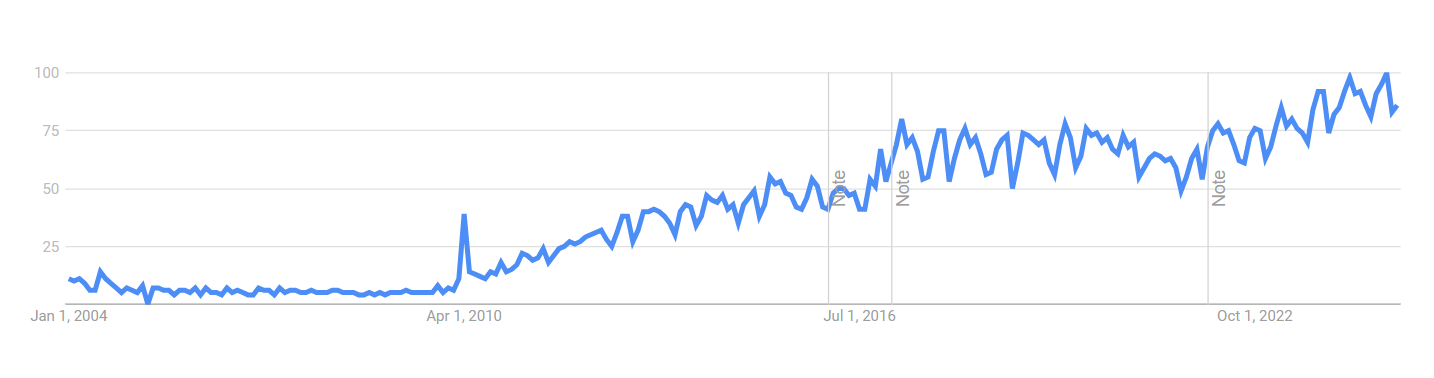
\includegraphics[width=\textwidth]{open_data_google_trends}
    \caption[Open Data su Google Trends]{Ricerche su Google relative al termine Open Data effettuate dal 2004 al 2025. Notare l'aumento successivo al 2009 e il trend in crescita \cite{Google_Trends}.}
    \label{fig:open_data_google_trends}
\end{figure}

\subsection{Concetto di Open Data}
%Definizione e principi fondamentali
Gli \textit{open data}, specialmente quelli della pubblica amministrazione, costituiscono una formidabile risorsa che ancora oggi rimane in larga parte inutilizzata. Molte persone e organizzazioni raccolgono una vasta gamma di svariati tipi di dati per svolgere le proprie attività. In questo ambito, il governo riveste particolare importanza, sia per la quantità e la centralità dei dati che raccoglie, sia perché la maggior parte dei dati del governo sono pubblici per legge, quindi potrebbero diventare aperti e resi disponibili per l'utilizzo da parte di chiunque. Questo riveste particolare interesse in quanto si ritiene che gli \textit{open data} possano apportare benefici in molti settori, ed esistono altrettanti esempi di come siano già stati usati con successo. Ci sono inoltre svariati gruppi di persone e organizzazioni che possono trarre vantaggi dalla disponibilità di \textit{open data}, incluso il governo stesso. Allo stesso tempo, è impossibile effettuare previsioni esatte su come e dove verranno apportati questi benefici in futuro, in quanto è nella stessa natura dell'innovazione che gli sviluppi spesso partano dai posti più inaspettati \cite{OpenDataHandbook_WhyOpenData}.

\subsection{Caratteristiche principali degli Open Data}
% Accessibilità, Interoperabilità, Riutilizzabilità
% Formati comuni: CSV, JSON, XML
In base a quanto stabilito dalla \textit{Open Definition}, gli \textit{open data} sono dati che possono essere utilizzati liberamente e ridistribuiti da chiunque e sono sottoposti, al massimo, al riconoscimento obbligatorio di una potenziale attribuzione o crediti in generale \cite{OpenDefinition}. Nella \textit{full Open Definition} vengono specificate in dettaglio le proprietà più importanti, ovvero:

\begin{itemize}
    \item \textbf{Disponibilità e Accesso:} i dati devono essere disponibili per intero, senza pagare più di un costo ragionevole di riproduzione, preferibilmente scaricandoli dalla rete Internet. I dati devono, inoltre, essere disponibili in un formato conveniente e modificabile.
    \item \textbf{Riutilizzo e Ridistribuzione:} i dati devono essere forniti sotto licenza che ne permetta liberamente il riutilizzo e la ridistribuzione, incluso specialmente il mescolamento con altri \textit{dataset}.
    \item \textbf{Partecipazione Universale:} tutti devono essere in grado di utilizzare, riutilizzare e ridistribuire i dati, senza discriminazioni contro campi di applicazione o contro persone o gruppi particolari. Ad esempio, non sono permesse le licenze ristrette ai soli scopi non-commerciali, che impedirebbero l'utilizzo commerciale, e nemmeno qualsiasi altra restrizione all'uso per certe finalità, come quella esclusivamente educativa.
\end{itemize}

Queste regole sono necessarie per garantire chiarezza sul significato di apertura e, soprattutto, per assicurarne l'\textit{interoperabilità}. Quest'ultima denota la capacità di lavorare insieme, ovvero interoperare, tra diversi sistemi e organizzazioni, che in questo caso si riferisce all'interoperabilità, detta anche mescolanza, tra dataset differenti. \`E una capacità molto importante perché permette a diversi componenti di collegarsi per lavorare insieme e questo è essenziale per realizzare sistemi grandi e complessi, la cui costruzione altrimenti sarebbe quasi impossibile senza interoperabilità \cite{OpenDefinition_Full}.

Il principio cardine di un \textit{commons} di dati o codice, ovvero una raccolta di essi, è che un qualunque pezzo di materiale aperto lì contenuto possa essere mescolato liberamente con altro materiale aperto. Questa interoperabilità è assolutamente necessaria a livello pratico per realizzare i principali benefici ottenibili dall'apertura dei dati, ovvero l'abilità notevolmente migliorata di combinare insieme diversi dataset e di conseguenza la capacità di sviluppare un numero maggiore di prodotti e servizi aventi qualità migliore. Questa definizione data riguardo all'apertura assicura che, dati due dataset aperti ottenuti da due fonti diverse, possiamo essere sempre in grado di combinarli insieme, evitando di trovarci di fronte a un numero enorme di dataset aventi scarsa o nulla capacità di essere mescolati insieme in sistemi di più larga scala, senza quindi avere la capacità di apportare valore aggiunto. Il punto chiave di aprire i dati deve essere il \textit{focus} su dati non-personali, ovvero i dati non devono contenere informazioni riguardanti persone specifiche. Inoltre, per alcuni tipi di dati ottenuti dal governo, potrebbero applicarsi restrizioni nazionali per motivi di sicurezza \cite{OpenDataHandbook_WhyOpenData}.

\subsection{Formati principali}
Gli open data possono essere utilizzati in svariati formati, di seguito vediamo quali.
\subsubsection{JSON}
Quello più utilizzato in ambito software è JSON, un semplice formato file che è molto facile da leggere per qualsiasi linguaggio di programmazione. La sua semplicità lo rende più veloce da processare per un computer rispetto ad altri formati come XML.
\subsubsection{XML}
XML è un formato molto utilizzato per lo scambio di dati, in quanto fornisce buone opportunità di mantenere la struttura dei dati e il modo in cui i file sono costruiti, permettendo agli sviluppatori di scrivere parti della documentazione insieme ai dati senza interferire con la loro lettura.
\subsubsection{RDF}
RDF è un formato raccomandato dal W3C e rende possibile rappresentare i dati in una forma in cui sono più facili da combinare con altri dati provenienti da più fonti. Dati RDF possono essere salvati in varie serializzazioni, tra cui XML e JSON. RDF incoraggia l'utilizzo di URL come identificatori, fornendo un modo conveniente di interconnettere direttamente iniziative open data già esistenti sul Web. Non è ancora molto diffuso, ma è diventato un trend tra le iniziative di Open Government, tra cui annoveriamo i progetti di Open Data collegati tra i governi di Regno Unito e Spagna. L'inventore di Internet, Tim Berners-Lee, ha recentemente proposto uno schema chiamato \textit{fivesstar} che include i dati RDF collegati, ponendolo come obiettivo da raggiungere per le iniziative di open data.
\subsubsection{\textit{Spreadsheet}}
Sono utilizzati da molte autorità, le quali hanno ancora delle informazioni rimaste in documenti come quelli di Microsoft Excel. Questi dati possono essere utilizzati immediatamente con la corretta descrizione del significato delle varie colonne. Tuttavia, in alcuni casi ci possono essere delle macro e delle formule nei fogli di calcolo, che possono diventare potenzialmente più complicate da gestire. Di conseguenza, è consigliabile documentare questo genere di calcoli di fianco allo \textit{spreadsheet}, dato che è generalmente più accessibile alla lettura da parte degli utenti.
\subsubsection{\textit{Comma-Separated Values}}
I file CSV possono essere un formato molto utile data la loro compattezza e possono quindi essere adatti al trasferimento di grandi quantità di dati all'interno della stessa struttura. Tuttavia, questo formato è talmente spartano che i dati sono spesso inutili senza appropriata documentazione, dato che può essere quasi impossibile indovinare il significato delle diverse colonne. Diventa quindi particolarmente importante che la documentazione dei singoli campi sia accurata. Inoltre, è essenziale rispettare la struttura del file, in quanto la singola omissione di un campo è in grado di disturbare la lettura di tutti i rimanenti dati del file senza avere una reale opportunità di aggiustamento, perché non si può determinare come vanno interpretati i dati rimanenti.
\subsubsection{Documento di testo}
I documenti classici in formati come Word, ODF, OOXML o PDF potrebbero bastare per mostrare alcuni tipi di dati, come delle \textit{mailing lists} relativamente stabili o equivalenti, senza richiedere un grande sforzo. Questo formato non offre alcun supporto per il mantenimento di una struttura coerente, il che spesso significa che diventa difficile inserire dati mediante strumenti automatizzati. Bisogna assicurarsi di utilizzare dei \textit{templates} come base dei documenti che mostreranno dati per il riuso, così da rendere possibile ottenere informazioni da tali documenti. Inoltre, per supportare ulteriormente l'utilizzo dei dati si potrebbero utilizzare dei \textit{markers} tipografici il più possibile, così da rendere più facile per una macchina la distinzione degli \textit{headings}, ovvero i titoli di qualsiasi tipo, dal contenuto, e così via. Generalmente è raccomandabile non esibirli in un formato di \textit{word processing}, se i dati esistono in formati differenti.
\subsubsection{Testo non formattato}
I documenti di testo non formattato (.txt) sono molto semplici da leggere per un computer, ma generalmente escludono metadati strutturali dall'interno del documento, quindi gli sviluppatori devono creare un \textit{parser} che possa interpretare ogni documento nell'ordine in cui appare. Possono verificarsi alcuni problemi dallo scambio di file \textit{plain text} tra diversi sistemi operativi, in quanto Windows, macOS e altre varianti Unix hanno ciascuno il loro modo di indicare al computer che si è raggiunta la fine della riga, quindi 3 diversi caratteri di \textit{newline}.
\subsubsection{Immagini scannerizzate}
Probabilmente questo è il metodo meno indicabile per la maggioranza dei dati, ma sia TIFF che JPEG-2000 sono in grado di dargli una documentazione di ciò che si trova nell'immagine, e possono addirittura indicare testualmente l'intero contenuto del documento all'interno di un'immagine dello stesso documento. Potrebbe essere rilevante mostrare dati come immagini i cui dati non sono stati creati elettronicamente, un esempio sono i materiali di archivio, per i quali avere un'immagine è sicuramente meglio di nulla.
\subsubsection{Formati proprietari}
Alcuni sistemi dedicati hanno i propri formati di dati con cui possono essere salvati o esportati. Talvolta può bastare esporre i dati in tale formato, specialmente se ci si aspetta che un ulteriore utilizzo avvenga in un sistema simile a quello da cui provengono. Va sempre indicato dove si possono trovare ulteriori informazioni su questi formati proprietari, per esempio fornendo un link al sito web del fornitore. Generalmente, se fattibile, è raccommandabile mostrare i dati in formati non-proprietari.
\subsubsection{HTML}
Al giorno d'oggi, molti dati sono disponibili in formato HTML su vari siti e questo potrebbe tranquillamente essere sufficiente se i dati sono molto stabili e con ambito limitato. In alcuni casi, però, potrebbe essere preferibile avere i dati in una forma più facile da scaricare e manipolare, ma dato che il riferimento a una pagina su un sito web è una modalità molto semplice ed economica, potrebbe costituire un buon punto di partenza nella visualizzazione di dati. Tipicamente, sarebbe più appropriato utilizzare delle tabelle in documenti HTML per contenere i dati, ed è importante che i vari campi di dati siano visualizzati e assegnati degli ID che li rendano facili da trovare e manipolare i loro dati. Per effettuare lo scraping, Yahoo ha sviluppato un \textit{tool} in grado di estrarre informazioni strutturate da un sito, e tali strumenti sono in grado di effettuare molte altre operazioni purché i dati siano accuratamente etichettati \cite{YahooDevelopers_YQL}.
\subsubsection{Formati Open File}
Anche se le informazioni sono fornite in formati elettronici, dettagliati e comprensibili da un computer (\textit{machine-readable}), potrebbero ugualmente verificarsi problemi relativi al formati del file stesso. I formati in cui le informazioni sono pubblicate, ossia la base digitale in cui le informazioni sono salvate, possono essere sia aperti che chiusi. Un formato aperto è uno in cui le specifiche per il software sono disponibili a tutti e in maniera gratuita, così che chiunque possa utilizzare queste specifiche nel loro software senza limitazioni al riuso imposte dai diritti sulla proprietà intellettuale. D'altro canto, se un formato file è chiuso, potrebbe essere sia perché è proprietario e le specifiche non sono disponibili al pubblico, o perché il formato file è proprietario ma il riuso è limitato, anche se le specifiche sono state rese pubbliche. Se le informazioni sono rilasciate in un formato chiuso, questo può causare ostacoli significativi al riuso delle informazioni in esso racchiuse, costringendo chi sia interessato a utilizzarle a comprare il software necessario. Il beneficio dei formati file aperti è che permettono agli sviluppatori di produrre più pacchetti software e servizi che utilizzano questi formati, minimizzando così gli ostacoli al riuso delle informazioni che contengono. Utilizzare formati file proprietari per i quali le specifiche non sono disponibili pubblicamente può generare una dipendenza su software di terze parti o sui detentori delle licenze del formato file, il che potrebbe significare, nello scenario peggiore, che sia possibile leggere le informazioni esclusivamente utilizzando certi pacchetti software, i quali potrebbero avere un costo proibitivo, o anche diventare obsoleti. Di conseguenza, per i dati aperti forniti dal governo vige la forte preferenza per cui le informazioni dovrebbero essere rilasciate in formati file aperti e \textit{machine-readable}, leggibili da un computer \cite{OpenDataHandbook_FileFormats}.

\subsection{Confronto con dati privati}
Differenze principali

Vantaggi e svantaggi rispetto agli Open Data

\subsection{Contesto italiano e internazionale}
Ad oggi, è già possibile indicare un cospicuo numero di settori nei quali i dati aperti del governo stanno già apportando un certo valore, tra cui:

\begin{itemize}
    \item Controllo di trasparenza e democrazia.
    \item Partecipazione.
    \item Autopotenziamento.
    \item Miglioramento o creazione di nuovi prodotti e servizi da parte di privati.
    \item Innovazione.
    \item Miglioramento dell'efficienza di servizi del governo.
    \item Miglioramento dell'efficacia di servizi governativi.
    \item Misuramento dell'impatto di certe politiche.
    \item Nuova conoscenza ottenuta dalla combinazione di fonti di dati e dalla ricerca di \textit{pattern} all'interno di grandi volumi di dati.
\end{itemize}

Riguardo alla trasparenza, esistono progetti come il finlandese \textit{tax tree}, l'albero delle tasse, e il britannico \textit{where does my money go}, dove vanno i miei soldi, per visualizzare in che modo i ricavi derivanti dalle tasse vengono spesi dal governo. Inoltre, possiamo ricordare come gli open data abbiano risparmiato al Canada \$3.2 miliardi in una frode fiscale relativa a un ente di beneficenza. Altri siti web includono il danese \textit{folketsting.dk} per tracciare l'attività in parlamento e i processi di creazione di leggi, così da poter vedere esattamente gli eventi che stanno accadendo, e quali parlamentari sono coinvolti.
Gli open data del governo possono anche aiutarci a prendere decisioni migliori nella nostra vita, o a diventare più attivi nella società. Una donna in Danimarca ha sviluppato \textit{findtoilet.dk}, che mostra tutti i bagni pubblici danesi così che le persone che conosceva con problemi alla vescica potessero diventare più sicuri di se stessi quando andavano nuovamente fuori. In Olanda è disponibile un servizio, \textit{vervuilingsalarm.nl}, che ci avvisa con un messaggio se domani la qualità dell'aria nelle vicinanze raggiungerà una soglia che abbiamo definito in precedenza. A New York possiamo facilmente capire dove possiamo portare il cane a passeggio, insieme a trovare altre persone che frequentano gli stessi parchi. Servizi come \textit{mapumental} nel Regno Unito e \textit{mapnificent} in Germania permettono di trovare dei posti in cui vivere, prendendo in considerazione la durata del tragitto per arrivare a lavoro, il prezzo delle case e la qualità di una certa zona. Tutti questi servizi, per funzionare, si appoggiano a dati forniti apertamente dal governo.
Economicamente, gli open data sono altrettanto importanti: diversi studi hanno stimato il valore economico degli open data in alcune decine di miliardi di Euro su base annua, e questo solamente nell'Unione Europea. Nuovi prodotti e aziende stanno riutilizzando dati aperti, come ad esempio il danese \textit{husetsweb.dk} che aiuta a trovare dei modi per migliorare l'efficienza energetica della propria casa, insieme alla pianificazione finanziaria e alla ricerca di costruttori che possano svolgere il lavoro. Tutto è basato sul riutilizzo delle informazioni catastali e informazioni sui sussidi da parte del governo, insieme al registro commerciale locale. Google Traduttore utilizza un enorme quantità di documenti dell'UE che compaiono in tutte le lingue europee per addestrare gli algoritmi di traduzione e quindi migliorare la sua qualità del servizio.
Gli open data offrono del valore anche al governo stesso, ad esempio per aumentarne l'efficienza. Il Ministero Olandese dell'Istruzione ha pubblicato online tutti i suoi dati relativi all'istruzione, permettendone il riuso. Da allora, il numero di domande che hanno ricevuto è crollato, riducendo il carico di lavoro e i relativi costi, mentre per i dipendenti pubblici è più facile rispondere alle rimanenti domande, in quanto diventa maggiormente chiaro dove possono essre trovate le informazioni rilevanti. Gli open data hanno anche reso più efficiente la pubblica amministrazione, il che porta a un'ulteriore riduzione dei costi. Il dipartimento olandese dei beni culturali sta rilasciando attivamente i loro dati e collabora con società amatoriali di storia e gruppi come la \textit{Wikimedia Foundation} per eseguire i loro compiti in maniera più efficiente. Questo non solo porta a miglioramenti nella qualità dei loro dati, ma contribuisce anche a rimpicciolire le dimensioni del dipartimento stesso.
Anche se ci sono già numerose istanze relative ai modi in cui gli open data stanno creando del valore aggiunto sia in ambito sociale che in quello economico, non sappiamo ancora nulla riguardo alle nuove cose che diventeranno possibili. Nuove combinazioni di dati possono creare ulteriore conoscenza, il che può potenzialmente portare a scoprire campi di applicazione completamente nuovi. Lo abbiamo già visto in passato, per esempio quando nel XIX secolo a Londra il Dott. Snow ha scoperto il legame tra inquinamento dell'acqua potabile e colera, combinando i dati delle morti attribuibili al colera con la posizione dei pozzi d'acqua. Questo portò alla costruzione dei sistemi fognari di Londra e migliorò notevolmente la salute pubblica della popolazione. Probabilmente potremmo vedere accadere nuovamente degli sviluppi simili, scaturiti dalla combinazione di diversi dataset aperti. Questo potenziale, ancora non sfruttato, può essere rilasciato se trasformiamo i dati pubblici del governo in open data, ma solo se sono davvero aperti, ovvero se non sottoposti ad alcun tipo di restrizione legale, finanziaria o tecnologica relativa al suo riutilizzo da parte di terzi. Ogni restrizione impedisce alle persone di riutilizzare i dati pubblici, o quantomeno lo rende più difficile. Per poter realizzare appieno il loro potenziale, i dati pubblici devono essere aperti, ovvero degli open data \cite{OpenDataHandbook_WhyOpenData}.

\subsubsection{Iniziative globali}
Open Government Partnership

\subsubsection{Normativa italiana}
CAD (Codice dell'Amministrazione Digitale)

\subsubsection{Portali di Open Data}
dati.gov.it

Open Data Bologna (https://opendata.comune.bologna.it/)

\subsubsection{Casi studio e iniziative significative}
INSPIRE

Copernicus


\section{Bologna e progetto BolognaWiFi}  %  e Comune di Bologna
\subsection{Bologna Smart City}
Il progetto di Bologna Smart City è iniziato il 30 luglio 2010, quando il Comune di Bologna, l'Alma Mater e Aster hanno firmato un Protocollo d'intesa per la realizzazione della relativa piattaforma, avente l'obiettivo di rispondere ai bisogni della comunità per migliorarne la qualità della vita e garantire i diritti fondamentali della socialità, dell'istruzione, dello sviluppo e della salute.
Le Smart Cities sono aree urbane intelligenti e sostenibili, in grado di pianificare in modo coerente l'integrazione delle diverse caratteristiche dell'identità del proprio territorio, siano esse economiche, produttive o ambientali, in un'ottica di innovazione.
Bologna ha scelto di intraprendere questo percorso per sviluppare soluzioni utili ad affrontare problematiche urbane e sociali, mettendo la tecnologia al servizio delle persone, attraverso un'alleanza tra mondo della ricerca, Università, imprese e pubblica amministrazione. Basandosi su questa definizione, la città di Bologna vuole essere pensata come un sistema intelligente e sostenibile dove si sfrutta l'ottimizzazione delle risorse per qualificare i servizi già esistenti e crearne di nuovi per costruire una città aperta alla partecipazione e al contributo creativo dei cittadini, ovvero il \textit{civic commons}, così come previsto dal Piano Strategico Metropolitano. Questo accordo sottoscritto ha anche lo scopo di implementare le attività svolte finora da Comune, Alma Mater e Aster sul tema delle Smart Cities ed è aperto all'adesione di altri enti e imprese.
Una città è intelligente se compie delle scelte nette e sostenibili, per cui bisogna investire con azioni strategiche nel campo di energia, servizi, digitale e valorizzazione dei beni ambientali e culturali. In questo ruolo, l'Università mette a disposizione i propri saperi, consapevole del suo legame storico con Bologna, figurandosi come un grande consulente sullo sviluppo della città, della società e dell'impresa. Bologna Smart City è un obiettivo prioritario affinché la regione Emilia-Romagna sia in grado di restare al passo con i tempi, in cui l'innovazione è fondamentale per la competitività imprenditoriale e per il sistema della ricerca, proprio a partire dalla rete di alta tecnologia.
In questo progetto, i tre partner (Comune, Università e Aster) hanno individuato un primo gruppo di 7 ambiti chiave su cui verteranno le azioni sui temi principali:
\begin{itemize}
    \item Beni Culturali: valorizza e riqualifica il centro storico e il suo patrimonio culturale, insieme ai portici e al turismo.
    \item Iperbole 2020 Cloud \& Crowd: riprogetta la Rete Civica Iperbole, basandosi sulla tecnologia cloud e un'identità digitale integrata, raccogliendo così l'offerta di contenuti e servizi di Pubblica Amministrazione, imprese e cittadini.
    \item Reti intelligenti: smart grid, banda ultralarga FTTH e smart lighting.
    \item Mobilità sostenibile: sviluppo di una rete della mobilità elettrica intelligente.
    \item Quartieri sicuri e sostenibili: ristruttura il patrimonio pubblico e privato per aumentare l'efficienza e la produzione di energia, monitora la sicurezza degli edifici, gestisce i rifiuti, configura il social housing, la domotica, il co-working, insieme a servizi e nuovi ambienti per lavoratori della conoscenza e ricercatori.
    \item Sanità e Welfare: e-care, e-health, ottimizzazione dei processi e business intelligence.
    \item Educazione e istruzione tecnica: sviluppo progetti in ambito educativo, promuove una nuova cultura tecnica e scientifica \cite{Bologna_Smart_City}.
\end{itemize}


Bologna è sempre di più una smart city e ha l'obiettivo di diventare una città sostenibile. Si trova già da anni ai primi posti delle classifiche delle smart city italiane. Una città che punta non solo ad essere inclusiva, sicura, attenta alla salute e all'ambiente, ma anche a fornire a tutti i suoi abitanti una serie di servizi tra cui in primis ci sono quelli della mobilità. Sappiamo che l'inquinamento atmosferico è un serio problema per la salute delle persone ed è legato alle emissioni, quindi una città smart sostenibile dovrebbe mettere a disposizione dei cittadini tutta una serie di sistemi volti a ridurre i livelli di CO\textsubscript{2}, particolato e altre sostanze pericolose. Nasce quindi il concetto di MaaS, Mobility as a Service, che consiste in una nuova idea di mobilità in cui si prevde l'integrazione dei vari servizi di trasporto pubblico e privato in un unico canale digitale, rendendoli più accessibili all'utente finale, e questa sharing mobility è già in sperimentazione a Milano. In questo modo, i cittadini possono scegliere tra varie soluzioni di mobilità sostenibile, configurandole come un'alternativa all'utilizzo dell'auto privata. A Bologna ne sono già un esempio il servizio di car-sharing elettrico e di bike-sharing, sia con biciclette classiche che con e-bike (biciclette a pedalata assistita): tutti questi servizi sono noleggiabili tramite una semplice app. Inoltre, a Bologna è attivo il servizio di Telepass Pay, che permette tramite app di pagare il parcheggio, prenotare un taxi, o prenotare la pulizia dell'auto e della moto nel punto in cui è parcheggiata. La tecnologia svolgerà sempre di più un ruolo fondamentale nella diffusione di questi servizi, sempre più diversificati e disponibili, permettendo al cittadino di scegliere il mezzo di trasporto più idoneo al tragitto da compiere e al contempo diminuendo il traffico in città, migliorando la qualità dell'aria e riducendo le emissioni \cite{Bolognatoday_Smart_City}.

\subsubsection{Digitalizzazione e innovazione urbana}
Progetti principali

\subsubsection{Politiche locali per gli Open Data}
Strategie e risultati

\subsubsection{Infrastrutture digitali recenti}
Implementazioni chiave

\subsection{Progetto BolognaWiFi}
Verso la fine degli anni '90, la rete Internet era sempre più diffusa e stava iniziando a diventare un'infrastruttura comunicativa, costituendo così una grande opportunità al servizio dei cittadini. Di conseguenza alcuni comuni italiani, tra cui quello di Bologna, riuscirono a comprenderne in maniera lungimirante le grandi potenzialità che offriva per costruire nuovi spazi di informazione, relazione e connessione civica.
Così nel 1995 il Comune di Bologna, in collaborazione con l'Alma Mater, creò la rete civica Iperbole, la quale venne pensata e sviluppata come una rete globale-locale. Questo progetto potè nascere proprio a Bologna in virtù di una rara situazione di privilegio riguardante l'innovazione amministrativa, molto più avanzata all'epoca rispetto alle altre città italiane.
La rete Iperbole offriva agli utenti la possibilità di avere accesso a Internet, fornendo anche un indirizzo email gratuito, e in questo modo ha saputo contribuire attivamente all'alfabetizzazione digitale dei cittadini bolognesi.
Iperbole è suddivisa in tre sezioni. Nella prima, quella del Comune, vengono riportate le iniziative e le attività svolte dal Comune di Bologna, così da permettere di rimanere aggiornati sulle tematiche correlate a Sindaco, Giunta, Consiglio Comunale, Elezioni, Turismo, Mobilità, Qualità dell'aria, Casa e Comunicati.
Nella seconda, quella dei Servizi Online, è possibile usufruire di tutti i servizi messi a disposizione dal Comune, come il pagamento di multe e bollettini MAV, la prenotazione per l'URP, la richiesta di un assegno familiare, la presentazione della dichiarazione ISEE e la segnalazione di problemi.
Nella sezione Partecipa, invece, il cittadino può impegnarsi e partecipare attivamente ai processi di collaborazione e cura dei beni comuni.
Negli ultimi anni il Comune di Bologna, in collaborazione con Lepida SpA, ha inaugurato la rete Iperbole Wireless, che offre a cittadini e visitatori un servizio di connessione a Internet tramite WiFi, che si configura come un'evoluzione \textit{mobile} della Rete Civica Iperbole. Tale rete wireless è aperta e non richiede autenticazione.
Dal 1995 ad oggi, Iperbole non è più solo una rete telematica di informazione costante e aggiornata per i cittadini, ma sta diventando un vero e proprio punto di riferimento grazie alla facilità di accesso e alle iniziative di partecipazione civica, rappresentando non solo una grande invenzione tecnologica, ma soprattutto un esempio di innovazione sociale grazie al quale si sono garantiti e messi in atto diritti digitali e di cittadinanza \cite{Iperbole_Citta_Connessa}.

Il Comune di Bologna, in collaborazione con Lepida spa, offre a cittadini e visitatori un servizio di connessione a internet in modalità Wi-Fi come evoluzione \textit{mobile} della Rete Civica Iperbole. Per navigare è sufficiente collegarsi alla rete BolognaWiFi, la quale è aperta e non richiede autenticazione. Nelle aree all'aperto è possibile accedere e navigare tutti i giorni 24 ore su 24, mentre nei luoghi all'interno di edifici si può navigare negli orari di apertura delle strutture che offrono il servizio. Ad oggi ci sono più di 300 hotspot attivi in città \cite{BolognaWiFi_Elenco_Hotspot}.


Già nel 2014, dopo un anno intero di operatività della connessione Wi-Fi pubblica a banda ultralarga, piazza Maggiore a Bologna era riuscita a ottenere il titolo di \textit{piazza più connessa d'Europa}, segno dell'importanza di questo progetto per la città felsinea \cite{Smart_City_Piazza_Connessa_Europa}.

BolognaWiFi è un servizio offerto dal Comune di Bologna e fornisce una connettività wireless gratuita a tutti i cittadini. Nato da una collaborazione con alcuni operatori nel settore delle telecomunicazioni, i primi test sono iniziati nel 2005 in Piazza Maggiore, insieme ad alcune ditte private che hanno aderito al progetto \cite{Bologna_WiFi_Bluetooth}.

\subsubsection{Obiettivi principali}
% Scopi e finalità del progetto
Tra gli obiettivi, Iperbole voleva garantire lo scambio di informazioni non soltanto tra le associazioni, ma anche tra individui, istituzioni e, in generale, con chiunque nel mondo avesse a disposizione un computer e un modem, favorendo forme di partecipazione e collaborazione civica.
Iperbole, tutt'oggi, rappresenta il tentativo di riprodurre in uno spazio digitale tutto quello che è lo spazio della città, creando situazioni di incontro e di confronto nella realtà più ampia che è quella di Internet. Queste realtà virtuali, dette anche agorà elettroniche con un riferimento alla piazza principale dell'antica Grecia, intendono rappresentare un punto di riferimento per il cittadino, una specie di mappa con cui orientarsi, informarsi e partecipare alle attività pubbliche della società \cite{Iperbole_Citta_Connessa}.


Lo scopo principale del progetto BolognaWiFi è quello di abbattere il \textit{digital divide}, agevolare la connettività mediante un servizio gratuito e, allo stesso tempo, favorire i cittadini nelle più svariate attività, a prescindere dal fatto che siano residenti, studenti, pendolari o turisti. L'idea originale era che si potesse navigare gratuitamente, sfruttando una miriade di utilità, tutto rimanendo seduti comodamente a uno dei bar del centro o all'ombra delle Due Torri \cite{Bologna_WiFi_Bluetooth}.


\subsubsection{Tipologie di dati raccolti}
% Flussi utenti
% Accessi WiFi
% Affluenza in aree urbane
Il servizio BolognaWiFi, come gli altri servizi di EmiliaRomagnaWiFi, nel corso del suo funzionamento raccoglie automaticamente alcuni dati personali dell'utente necessariamente correlati alle attività tecniche strumentali alla resa del servizio in questione. In particolare, sono trattati:
\begin{itemize}
    \item Timestamp di richiesta o di rinnovo o di cessazione dell'indirizzo IP alla rete da parte del dispositivo mobile.
    \item Indirizzo IP intranet assegnato al dispositivo mobile dalla rete.
    \item Identificativo MAC address del dispositivo mobile immediatamente pseudonimizzato con opportuni algoritmi non invertibili.
\end{itemize}
L'indirizzo IP intranet assegnato viene utilizzato in tutti i punti di accesso che fanno capo ad una stessa rete. La dimensione di una rete varia a seconda dei territori, ma tipicamente è costruita in modo da includere almeno tre diversi punti di accesso.
Il trattamento dei dati è necessario per l'esecuzione di compiti di interesse pubblico o connessi all'esercizio di pubblici poteri di cui è investita la regione Emilia-Romagna e non necessita di un consenso. Nello specifico, all'interno del servizio BolognaWiFi (EmiliaRomagnaWiFi) i dati personali acquisiti vengono trattati per lo svolgimento di funzioni istituzionali e, in particolare, è finalizzato a offrire il servizio di WiFi a banda ultra larga, pubblico, libero, senza autenticazione e gratuito, monitorandone il corretto funzionamento al fine di assicurarne qualità, continuità e accessibilità.
I dati personali acquisiti sono trattati, con strumenti informatici, rispettando i principi stabiliti dalla normativa vigente, attraverso modalità idonee a garantire la riservatezza e la sicurezza dei dati. In particolare, vengono rispettati i principi di liceità, correttezza, trasparenza, limitazione delle finalità, minimizzazione dei dati, esattezza, limitazione della conservazione, integrità e riservatezza, e responsabilizzazione stabiliti dal GDPR. Il trattamento di aggregazione ed elaborazione per fini statistici viene effettuato su dati pseudonimizzati e qualsiasi statistica puntuale viene prodotta se coinvolge almeno tre diversi dispositivi mobili. I dati raccolti non consentono di identificare la posizione del dispositivo mobile tra i punti di accesso che fanno parte della stessa rete. Diventa quindi impossibile procedere a una reidentificazione dell'interessato, a meno che tale soggetto non lo richieda direttamente, indicando il proprio MAC address. Anche in questo caso, ciò è possibile solamente se tale indirizzo non è stato rigenerato casualmente dal sistema operativo del dispositivo mobile. I dati personali non sono oggetto di comunicazione o diffusione e non sono mai trasferiti al di fuori dell'Unione Europea. Rimane il fatto che il conferimento dei dati non sia obbligatorio \cite{Informativa_EmiliaRomagnaWiFi}.

A partire da questi dati grezzi vengono poi ricavati dati più elaborati in forma aggregata su base giornaliera, come:
\begin{itemize}
    \item Matrice spostamenti: totale degli spostamenti orari delle persone da e verso ciascuna zona coperta da WiFi pubblico \cite{BolognaWiFi_Spostamenti}.
    \item Affluenza: viene registrato il numero di dispositivi che sono entrati in una data area coperta da WiFi pubblico, per ogni ora del giorno \cite{BolognaWiFi_Affluenza}.
    \item Affollamento: viene registrato il numero di dispositivi che sono presenti in una certa zona coperta da WiFi pubblico, per ogni ora del giorno \cite{BolognaWiFi_Affollamento}.
    \item Connessioni giornaliere: viene registrato il totale di connessioni giornaliere al servizio di WiFi pubblico BolognaWiFi. Uno stesso dispositivo che si collega più volte al servizio nell'arco di 24 ore viene contato una volta sola \cite{BolognaWiFi_Connessioni_Giornaliere}.
\end{itemize}
Oltre a questi dati, vengono salvati anche l'elenco di hotspot \cite{BolognaWiFi_Elenco_Hotspot} assieme all'elenco di aree coperte da segnale del BolognaWiFi \cite{BolognaWiFi_Elenco_Aree_Segnale}.

\subsubsection{Statistiche recenti}
Dati sull'uso del WiFi pubblico a Bologna

\subsubsection{Risorse utili}
Documentazione ufficiale del progetto

Report e analisi pubblicati dal Comune


\section{Visualizzazione dei dati}  % Analisi e
\subsection{Importanza della visualizzazione}
La \textit{data visualization} consente alle Città di comunicare facilmente con i Cittadini, visualizzando le città e le loro dinamiche attraverso strumenti capaci di trasformarle in rappresentazioni grafiche o schematiche. In questo modo, si offrono ai cittadini informazioni rapide ed esaustive per costruire un dialogo con l'amministrazione, facendo della Data Visualization una grande opportunità per città sempre più smart.
Nel mondo, il 90\% dei dati circolanti è stato generato negli ultimi due anni. Ogni giorno generiamo globlamente 2.5 EB (Exabytes) di nuovi dati e colleghiamo alla rete circa 1000 miliardi di dispositivi e oggetti a livello globale, creando un ambiente davvero favorevole all'Internet of Things (IoT).
La data visualization, detta anche visualizzazione dati, è la rappresentazione dei dati in formato grafico o comunque visivo, la quale permette di analizzare grandi quantità di dati, ovvero i Big Data, in modo semplice, tramite grafici e rappresentazioni più comprensibili di una lista grezza di dati. Data la nostra scarsissima soglia di attenzione, che secondo gli ultimi rilievi si attesta a circa 8 secondi, questa tecnica diventa importantissima data la grande disponibilità di informazioni che possediamo. Le rappresentazioni grafiche più semplici sono anche quelle più riuscite, e al contempo le più potenti.
Le nostre città generano continuamente dei dati, basta considerare la tradizionale urbanistica, i flussi di traffico, la disponibilità di parcheggio, la qualità dell'aria, la gestione energetica e la sensoristica avanzata. I sistemi informativi territoriali offrono da molto tempo un sistema per analizzare velocemente questi dati, capaci di evolvere velocemente nel tempo e fornire agli amministratori delle informazioni in modo rapido ed efficace. Tra tutte queste tecniche di elaborazione di dati e visualizzazione, alcune sono ormai canonizzate e considerabili \textit{commodity}, ma dall'arrivo di Google Maps e della presenza ubiquitaria di strumenti di localizzazione abbiamo una nuova ondata di \textit{location awareness} da parte degli utenti finali, siano essi cittadin residenti, turisti o businessmen, che può essere utilizzata dalle amministrazioni per migliorare il dialogo tra pubblico e privato.
Per esempio, affermare che l'impatto del cambiamento climatico stia rendendo più complessa la vivibilità delle città, o che entro 30 anni le città accoglieranno più di 2.5 miliardi di persone, è diverso dal mostrare una mappa della stessa città con l'andamento delle temperature medie nel tempo per ogni zona, o una mappa dell'Italia avente i flussi migratori in entrata e uscita, sia interni che esterni.
Riguardo alle applicazioni \textit{business to business}, o B2B, la data visualization ha un forte impatto in quanto permette di analizzare i fenomeni in modo multidimensionale dove la localizzazione geografica può avere un forte impatto e consente quindi la comprensione di situazioni che sarebbero difficili da analizzare mediante una visione tabellare del fenomeno.
Inoltre, per via del modo in cui il cervello umano elabora le informazioni, per visualizzare grandi moli di dati è più efficace e comprensibile impiegare mappe, grafici, illustrazioni o combinazioni di questi, rispetto all'utilizzo di fogli di calcolo o report.
La data visualization, oltre alla facilità di comprensione, permette:
\begin{itemize}
    \item Riconoscimento di pattern nei dati in modo intuitivo e veloce.
    \item Rapida identificazione degli outlier, ossia gli elementi che non seguono nessun trend particolare.
    \item Comprensione di fattori che influenzano i fenomeni.
    \item Predizione di fenomeni e trend \cite{DataVisualization_Citta}.
\end{itemize}

\subsubsection{Analisi dei dati urbani}
Esempi pratici e benefici

\subsubsection{Supporto decisionale}
Impatti sulle amministrazioni pubbliche

Si dice che \textit{un'immagine vale più di mille parole} e oggi, nell'era dei big data, con le aziende che vengono inondate da informazioni provenienti da vari tipi di dati e fonti on-premise e cloud-based, quel detto non potrebbe essere più vero. Filtrare le informazioni per distinguere quelle utili da quelle inutili sta diventando un compito sempre più arduo, ma le visualizzazioni rendono l'analisi molto più semplice e veloce, in quanto basta una sola occhiata per trovare le informazioni utili. Inoltre, noi umani sappiamo rispondere molto meglio alle visualizzazioni rispetto che al testo, dato che il 90\% delle informazioni inviate al cervello è di tipo visivo e il cervello elabora gli elementi visivi 60 000 volte più velocemente rispetto a quelli testuali. Di conseguenza, capiamo come la visualizzazione dati possa offrire benefici per l'analisi e la trasmissione di informazioni.
La visualizzazione dei dati genera impatto, fa parte di molti strumenti di business intelligence, ed è fondamentale per ottenere Advanced Analytics. Permette alle persone di trovare un senso in tutte le informazioni o dati generati oggi. Grazie alla data visualization, le informazioni vengono rappresentate in forma grafica, mediante un grafico a torta, un diagramma o altri tipi di presentazione visuale.
I visual analytics sono importanti perché una buona visualizzazione dei dati è fondamentale per poterli analizzare e prendere decisioni mirate, ptermettendo così alle persone di vedere e comprendere in modo semplice e rapido dei modelli e relazioni, individuando trend emergenti che potrebbero passare inosservati se presentati solo in una tabella o in un foglio di calcolo contenente numeri non elaborati. Generalmente non è richiesta alcuna formazione specializzata per interpretare il contenuto dei grafici, quindi possiamo ottenere una comprensione universale. Un grafico ben progettato non offre solo informazioni, ma riesce anche ad aumentare l'impatto di quest'ultime grazie a una presentazione forte, che attira l'attenzione e suscita interesse in un modo che nessuna tabella o foglio di calcolo sarebbe in grado di fare.
La maggior parte degli strumenti di visualizzazione dei dati è in grado di connettersi con fonti di dati, come i database relazionali. Questi dati possono essere archiviati on-premise o nel cloud e vengono recuperati per l'analisi. Gli utenti possono selezionare il modo migliore per presentare i dati da numerose opzioni. Alcuni strumenti forniscono automaticamente consigli di visualizzazione in base al tipo di dati presentati.
Un grafico dovrebbe prendere sempre in considerazione il tipo e lo scopo dei dati, in quanto alcune informazioni si adattano meglio a un tipo di grafico rispetto che a un altro, per esempio un grafico a barre invece di un grafico a torta. Con la maggior parte degli strumenti, l'utente ha una vasta scelta di opzioni di analytics visuali, da diagrammi comuni come grafici a linee e a barre, fino a sequenze temporali, mappe, tracciati, istogrammi e design personalizzati.
La visualizzazione dei dati può aiutare a raccontare la storia, trasmettendo in modo chiaro problemi complessi. Può svolgere un ruolo chiare nell'identificazione delle informazioni significative estraendole dal rumore, includendo sia anomalie che eccezioni. Inoltre, è in grado di aiutare con il crescente volume di dati, dato che l'interazione visuale con grandi dataset può semplificare l'analisi, rivelando nuovi insight. Tutto questo è permesso dalla visualizzazione dei dati, ma è necessario scegliere lo strumento giusto \cite{Oracle_Visualizzazione_Dati}.

\subsection{Caratteristiche di una buona visualizzazione}
% Chiarezza e semplicità
% Interattività e Accessibilità
La disciplina della Visualizzazione Dati è in continua evoluzione, dato l'uso sempre più ampio in un numero di campi sempre maggiore. All'inizio era solamente possibile trasformare i dati in grafici statici, ma oggi l'evoluzione ha portato a possiblità straordinarie.
Per costruire una buona visualizzazione dati, ci sono tre aspetti fondamentali:
\begin{enumerate}
    \item La visualizzazione deve essere efficace.
    \item Deve evidenziare ed esplicare i dati e le connessioni tra dati troppo difficili da spiegare con sole parole.
    \item Deve rendere facilmente comprensibili a chiunque sia le informazioni presentate, sia le possibili soluzioni al problema che si sta presentando.
\end{enumerate}
Ne è un esempio la seguente visualizzazione in Figura~\ref{fig:nintendo_sales} relativa alle vendite della console Nintendo Switch \texttrademark nel corso del tempo, ripartite tra software e hardware.
\begin{figure}
    \centering
    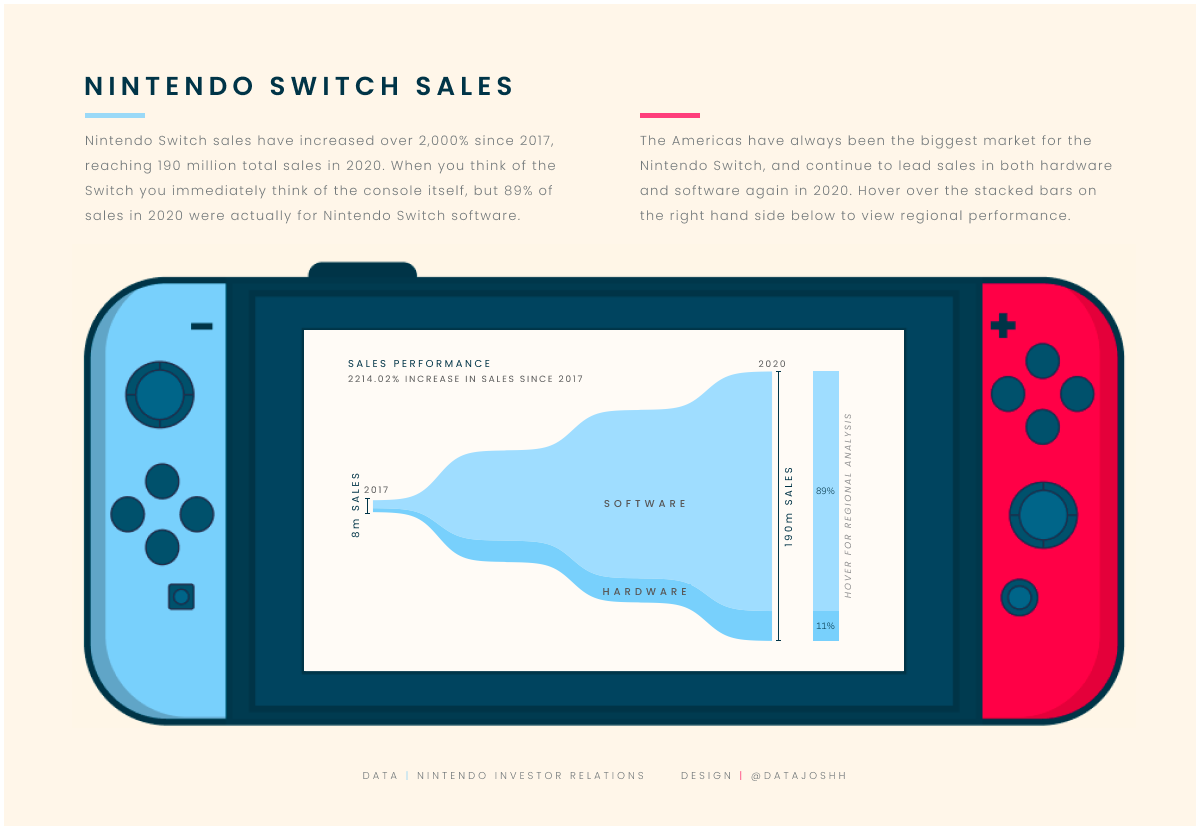
\includegraphics[width=\textwidth]{nintendo_sales.png}
    \caption[Dataviz: vendite di console Nintendo Switch]{Quando pensiamo alla Nintendo Switch \texttrademark, la prima cosa che viene in mente è la console stessa. Tuttavia, i dati ci mostrano che l'89\% delle vendite nel 2020 hanno riguardato software compatibile con la console, e non il relativo hardware \cite{DataVisualization_Caratteristiche}.}
    \label{fig:nintendo_sales}
\end{figure}
Queste regole di base sono molto generiche, ma devono restare una necessità sia quando di dati da gestire e presentare sono tanti, sia quando sono pochi. La complessità del lavoro non deve far desistere dal seguire queste linee guida, al contrario, maggiore è la mole di dati e più si rivela necessario seguire queste regole per arrivare a un buon risultato.
La prima cosa da fare quando si pensa a una visualizzazione dati è capire esattamente qual è il messaggio che vogliamo trasmettere, e con quali dati. Inoltre, è molto importante avere chiaro qual è il tipo di utente che utilizzerà la nostra dashboard, per evitare di presentare informazioni giuste alle persone sbagliate, e viceversa. Per esempio, all'interno di un'azienda è molto difficile il direttore finanziario sia interessato ai \textit{conversion rate} delle ultime campagne di marketing, ma è molto più probabile che sia interessato alla spesa di queste campagne messa in relazione con i profitti che ha generato.
Solitamente la complessità del lavoro deriva dal numero di variabili che entrano in gioco, di conseguenza è cruciale scegliere il tipo di grafico giusto.
In generale, i grafici a torta o a ciambella sono da evitare se le variabili sono più di 3, poiché si arriva a un punto dove la visualizzazione non è più efficace e non riesce a trasmettere in modo chiaro il messaggio. Una distribuzione statistica di alcune variabili rappresentata con un tale grafico a torta, per esempio, sarebbe pressoché inutile, dato che l'utente non riuscirebbe a capire il messaggio. AL contrario, per la stessa visualizzazione della distribuzione statistica su dati numerici, sarebbe molto più adatto un istogramma, o un box plot, se abbiamo interesse nelle sue modalità e valori anomali.
Riguardo ai colori, è significativo utilizzarli nel modo appropriato: nbel caso di una distribuzione statistica, in presenza di valori anomali o \textit{outliers}, per metterli in evidenza è consigliabile utilizzare dei colori accesi, così da farli risaltare e permettergli di comunicare già dei concetti in maniera autonoma. Per esempio, un mese dell'anno avente ricavi al di sopra della media potrebbe essere evidenziato in verde, colore che richiama un'idea positiva, mentre un mese avente costi fuori dalla media potrebnbe essere etichettato in rosso, per indicarne la negatività. In alternativa, potremmo anche utilizzare diverse sfumature dello stesso colore, assegnando una sfumatura intensa per i dati maggiori e una più tenue per quelli minori.
Un'ottima visualizzazione dovrebbe ridurre la complessità insita nelle tante variabili dei dati e, nel caso si dovessero compiere delle scelte, queste devono sempre aiutare il processo decisionale. In un progetto complesso invece è ancora più indicato se i dati vengono presentati in modo gerarchico, seguendo le priorità aziendali.
In generale, a prescindere dalle variabili e dalle osservazioni disponibili, basta seguire alcune regole pratiche per trasformare le visualizzazioni in un mezzo potente per illustrare il concetto alla base dei dati. Ne esistono tantissime, ma queste sono quelle principali:
\begin{itemize}
    \item Il colore del grafico non deve essere in contrasto con il background.
    Lo sfondo dovrebbe essere abbastanza neutro, così da garantire la massima libertà in termini di sfumature e colori per i grafici. Bisogna inoltre tenere in mente il fatto che le dashboard potrebbero venire stampare, quindi un utilizzo eccessivo del nero sullo sfondo potrebbe essere controindicato.
    \item Ogni variabile dovrebbe avere dei punti di riferimento, quando necessario.
    Per esempio, se forniamo i dati in termini di vendita per l'anno corrente, non tutti potrebbero essere in grado di discernere se si tratti di performance buone o cattive, indipendentemente dal fatto che la curva sia in crescita o in decrescita. Se invece mostriamo anche i dati delle vendite dello scorso anno, possiamo creare un punto di riferimento in grado di aiutare chiunque a capire meglio il significato del grafico.
    \item I grafici a barre vanno etichettati con i numeri, ma non eccessivamente.
    Bisogna aggiungere solo le indicazioni strettamente necessarie per far comprendere, tenendo a mente che i numeri lunghi sono generalmente difficili da visualizzare e che, se la precisione del dato non è indispensabile, è consentito e anzi consigliato arrotondare. Ad esempio, il valore \textit{10 523} può essere arrotondato a \textit{10K}, incrementando la chiarezza e riducendo la complessità.
    \item I dati vanno ordinati per enfatizzare la scala ove possibile, ma bisogna fare attenzione a non trasmettere un messaggio sbagliato.
\end{itemize}
La regola generale è che, minore è il quantitativo di dati che utilizziamo nelle visualizzazioni, maggiore è la chiarezza di quella risultante. Bisogna lavorare con l'essenziale in termini di grafica \cite{DataVisualization_Caratteristiche}.

\subsection{Strumenti di visualizzazione}
\subsubsection{Panoramica degli strumenti comuni}
Tableau

D3.js

\subsubsection{Vantaggi e svantaggi degli strumenti}
Breve descrizione comparativa

\subsubsection{Applicazioni pratiche: dati sul traffico in Regno Unito}
% Esempi nelle smart cities
Andrew Nicolson è uno sviluppatore software che è stato coinvolto in una campagna di successo contro la costruzione di una nuova strada, la \textit{Westbury Eastern bypass}, nel Regno Unito. Nell'aprile 2010, Andrew era interessato a ottenere accesso e a utilizzare i dati sul traffico della strada che stavano venendo utilizzati per giustificare le proposte e così è riuscito a ottenere alcuni dei dati rilevanti mediante la libertà di richieste di informazioni, ma il governo locale gli ha fornito i dati in un formato proprietario che può essere letto solamente utilizzando software prodotto da un'azienda chiamata Saturn, che è specializzata in modellazione di traffico e sulle relative previsioni. Non esiste una versione del software di sola lettura, quindi il gruppo di Andrew non aveva altra scelta se non acquistare una licenza software, finendo per pagare £500 (€600) utilizzando uno sconto per studenti. Il pacchetto software principale veniva offerto da Saturn a partire da £13\ 000, oltre €15\ 000, un prezzo fuori misura per la maggioranza dei normali cittadini. Anche se nessuna legge nel diritto dell'informazione garantisce un diritto ad avere l'accesso ai dati in formati aperti, le iniziative open data del governo stanno iniziando ad essere accompagnate da documenti di \textit{policies} che stabiliscono che le informazioni ufficiali debbano essere rese disponibili in formati di file che siano aperti. L'amministrazione Obama ha definito il \textit{gold standard}, con la \textit{Open Government Directive} emessa nel dicembre 2009, la quale decreta che, nella misura praticabile e soggetta a restrizioni valide, le agenzie debbano pubblicare informazioni online in un formato aperto che possa essere recuperato, scaricato, indicizzato e ricercato da applicazioni di ricerca web di utilizzo comune. Un formato aperto è inteso come uno che sia indipendente dalla piattaforma, leggibile dalla macchina e reso disponibile al pubblico senza restrizioni che impediscano il riuso di tali informazioni \cite{OpenDataHandbook_FileFormats}.


\section{Sfide e opportunità}   % Benefici e potenziale degli Open Data
\subsection{Sfide tecniche}
\subsubsection{Gestione di dataset eterogenei}
Problemi e soluzioni

\subsubsection{Scalabilità e performance}
Tecnologie per ottimizzare

\subsection{Aspetti etici e legali}
Quando parliamo di database, dobbiamo innanzitutto effettuare una distinzione tra la struttura e il contenuto: utilizzando il termine \textit{dati} ci riferiamo al contenuto del database, mentre gli elementi strutturali fanno riferimento ad attributi come i nomi dei campi e il modello della struttura dati, ovvero l'organizzazione dei campi sopra citati e le loro interrelazioni. In molte giurisdizioni è probabile che gli elementi strutturali di un database siano coperti da copyright, anche se ciò dipende in una certa misura dal livello di creatività che è stato coinvolto nella creazione della struttura. Tuttavia, in questo caso siamo particolarmente interessati ai dati. Quando parliamo di dati dobbiamo prestare attenzione, in quanto tale parola non è particolarmente precisa e può riferirsi sia a un insieme che a un singolo elemento, ma può anche significare una grande raccolta di dati, come tutto il contenuto del database. Per evitare confusione, riserveremo il termine \textit{contenuto} per riferirci ai singoli elementi, mentre la parola \textit{dati} riguarderà l'intera raccolta. Diversamente da materiali multimediali come testi, musica o film, la situazione legale per i dati varia notevolmente tra diversi Paesi. Tuttavia, la maggior parte delle giurisdizioni gli garantisce alcuni diritti in qualità di raccolta dati. La distinzione tra il contenuto del database e l'intera raccolta diviene particolarmente cruciale per i database fattuali, dato che nessuna giurisdizione garantisce il diritto di monopolio sui fatti individuali, ovvero il contenuto, anche se potrebbe garantire loro dei diritti in qualità di raccolta dati. Per fare un esempio, consideriamo un semplice caso di un database che elenca i punti di fusione di varie sostanze. Mentre l'intero database potrebbe essere protetto dalla legge, così da non permettere a nessuno di accedere, riusare o ridistribuire i suoi dati senza averne il permesso, questo non impedirebbe mai a nessuno di affermare il fatto che la sostanza Y si scioglie alla temperatura Z. Le forme di protezione per le raccolte dati ricadono largamente in due casi: diritto d'autore e diritto \textit{sui generis}. Come abbiamo già sottolineato, non abbiamo nessuna regola generale e la situazione varia in base alla giurisdizione. Di conseguenza, bisogna procedere considerando singolarmente ciascun Paese per delineare, se applicabile, quale dei due approcci sia utilizzato in una particolare giurisdizione. Dobbiamo inoltre notare come, in assenza di protezione legale, molti fornitori di database chiusi, ovvero non aperti, possono utilizzare un semplice contratto combinato con disposizioni legali per proibire la violazione dei meccanismi di controllo dell'accesso e ottenere così dei risultati simili a quelli dati da un diritto formale sull'indirizzo IP. Ad esempio, il provider di un database di citazioni può raggiungere qualsiasi insieme di termini e condizioni che voglia implementare, semplicemente richiedendo agli utenti di autenticarsi tramite una password, o fornendo agli utenti un account e una password alla condizione che l'utente accetti i termini e le condizioni del servizio \cite{OpenDataHandbook_LegalRights}.


\subsubsection{Privacy e anonimizzazione dei dati}
Strumenti e tecniche utilizzate

\subsubsection{Licenze e diritti d'uso}
Regolamenti e pratiche comuni

\subsubsection{Casi noti di violazioni}
Esempi significativi e lezioni apprese


\subsection{Opportunità}
\subsubsection{Trasparenza e coinvolgimento}
Benefici per cittadini e istituzioni

\subsubsection{Pianificazione urbana}
Utilizzo dei dati per migliorare i servizi

\subsubsection{Collaborazioni pubblico-privato}
Partnership per sfruttare al meglio gli Open Data

% \subsection{Fonti per approfondire}
% \subsubsection{Linee guida GDPR}
% Applicazioni rilevanti per i dati urbani

% \subsubsection{Studi accademici}
% Temi su etica e Open Data